%!TEX root = ../thesis.tex
%*******************************************************************************
%****************************** Second Chapter *********************************
%*******************************************************************************

\chapter{STUDI PUSTAKA}

\ifpdf
    \graphicspath{{Chapter2/Figs/Raster/}{Chapter2/Figs/PDF/}{Chapter2/Figs/}}
\else
    \graphicspath{{Chapter2/Figs/Vector/}{Chapter2/Figs/}}
\fi

Elektrokardiografi (ECG atau EKG) merupakan metode standar yang paling umum digunakan dalam dunia medis untuk mengukur tingkat HR dan BR pada tubuh.~Menghitung HR dan BR secara manual juga merupakan cara yang sering dilakukan.~Namun, penelitian sebelumnya telah menunjukkan bahwa metode manual ini cenderung tidak dapat diandalkan dalam perawatan pasien akut, dan dibatasi oleh keahlian pengukuran dokter [\citet{hillman2005}].~Oleh karena itu, dikembangkan metode \textit{Photoplethysmography} (PPG) yang memanfaatkan karakteristik gelombang cahaya untuk memonitor tingkat HR dan BR.~Berdasarkan Sun dan Thakor \citep{sun2016}, metode PPG dikelompokkan menjadi dua, yaitu (a) kontak, dan (b) non-kontak.~Metode PPG dengan kontak dapat disebut juga dengan istilah \textit{wearable} PPG karena prosesnya yang memerlukan kontak langsung antara sensor yang digunakan dengan bagian tubuh tertentu.~Sementara itu, metode non-kontak PPG dapat disebut dengan istilah \textit{non-wearable} PPG karena tidak memerlukan kontak langsung antara sensor dengan bagian tubuh tertentu dalam prosesnya.



%Penelitian sebelumnya untuk melakukan monitor denyut jantung (HR) dan tingkat pernapasan (BR) menggunakan sensor \textit{non-wearable} contohnya kamera \textit{Charge-Coupled Device} (CCD) [\citet{Allen2007,Estepp2014,Wu2000}], kamera RGB [\citet{deHaan2013,Mirmo2016,Poh2010,Poh2011}] serta smartphone [\citet{lazaro2014,nam2014}]. Penggunaan kamera maupun smartphone untuk memonitor HR dan BR cenderung berfokus pada bagian tubuh tertentu misalnya kepala ataupun warna kulit kepala. Dalam praktisnya hal ini sulit untuk diterapkan karena metode tersebut hanya khusus untuk karakteristik bagian tubuh tertentu, dan penempatan posisi kamera terlihat kurang praktis karena menggunakan kamera sejenis smartphone. 

\section{Karakteristik Gelombang Cahaya Pada Kulit}

Interaksi antara cahaya dengan jaringan biologis bisa sangat kompleks dan mungkin melibatkan aktifitas seperti penyebaran, penyerapan dan atau pantulan cahaya.~Penelitian Anderson dan Parrish \citep{ANDERSON1981} memeriksa karakteristik optis dan penetrasi cahaya pada kulit manusia.~Dalam wilayah kulit yang tampak, puncak penyerapan cahaya dominan mirip dengan nilai spektrum cahaya biru, kemudian diikuti dengan wilayah spektrum cahaya hijau-kuning ---antara 500nm hingga 600nm--- yang mempunyai karakteristik mirip dengan sel darah merah.~Panjang gelombang yang lebih pendek akan diserap oleh melanin.~Air menyerap cahaya ultraviolet dan spektrum cahaya yang lebih panjang dari spektrum IR, sedangkan spektrum cahaya merah dan inframerah (IR) dapat dilewatkan dengan mudah.~Oleh karena itu, panjang gelombang IR dapat digunakan sebagai sumber cahaya dalam sensor PPG.~Darah menyerap lebih banyak cahaya daripada jaringan tubuh lain di sekitarnya.~Oleh karena itu, pengurangan jumlah darah dapat diidentifikasi sebagai peningkatan intensitas cahaya yang terdeteksi. 
\newpage
\begin{figure}[ht]
	%\vspace{0.5em}
	\centering
	\includegraphics[width=0.9\textwidth]{light}
	\caption{Ilustrasi penetrasi cahaya dalam kulit.}
	\captionsetup{font={footnotesize}}  
	\caption*{sumber: Ash, C. et al. (2017). "Effect of wavelength and beam width on penetration in light-tissue interaction using computational methods." \textit{Lasers in Medical Science,} Vol.~32, halaman 1910.}
	\label{fig:light}   
\end{figure}

Gambar~\ref{fig:light} menunjukkan bahwa panjang gelombang menentukan seberapa jauh penetrasi cahaya dalam kulit.~Selain itu, jarak antara sumber cahaya dengan fotodetektor juga merupakan faktor yang penting.~Spektrum cahaya hijau cocok digunakan untuk pengukuran aliran darah superfisial (wilayah luar) kulit.~Cahaya dengan panjang gelombang antara 500 dan 600 nm menunjukkan kedalaman modulasi terbesar dengan penyerapan cahaya oleh aktifitas pulsatil darah.~Panjang gelombang IR atau yang mendekati IR lebih baik untuk pengukuran aliran darah di dalam jaringan.~Misalnya pengukuran aliran darah di otot.~Hal tersebut membuat IR marak digunakan pada perangkat PPG selama beberapa waktu [\citet{Tamura2014}].~Namun dalam beberapa tahun terakhir penggunaan spektrum warna hijau dalam perangkat PPG semakin populer karena intensitas variasi yang besar dalam modulasi yang diamati selama siklus jantung untuk panjang gelombang hijau [Jonathan dan Leahy \citep{Enock}, \citet{Lee2013,Maeda2011,Maeda2008,Matsu2014,Scully2012}].
LED hijau memiliki daya serap yang jauh lebih besar untuk oksihemoglobin dan deoksihemoglobin dibandingkan dengan cahaya inframerah.~Oleh karena itu, perubahan dalam cahaya hijau yang dipantulkan lebih besar dari pada cahaya inframerah yang dipantulkan ketika darah menembus kulit, menghasilkan rasio signal dengan gangguan yang lebih baik untuk sumber cahaya hijau [\citet{Tamura2014}].


%\section{Macam Macam Metode Pengukuran HR dan BR}
\section{Elektrokardiografi (ECG atau EKG)}

\begin{figure}[ht]
	\vspace{0.5em}
	\centering
	\begin{subfigure}[b]{0.49\textwidth}
		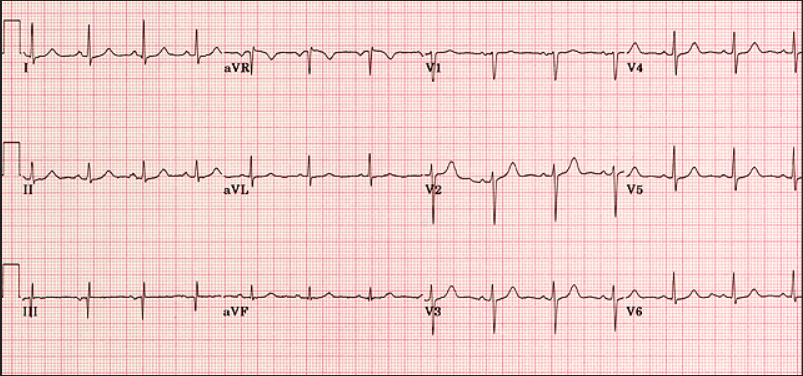
\includegraphics[width=\textwidth]{Normal_ECG}
		\caption{}
	\end{subfigure}             
	\begin{subfigure}[b]{0.49\textwidth}
		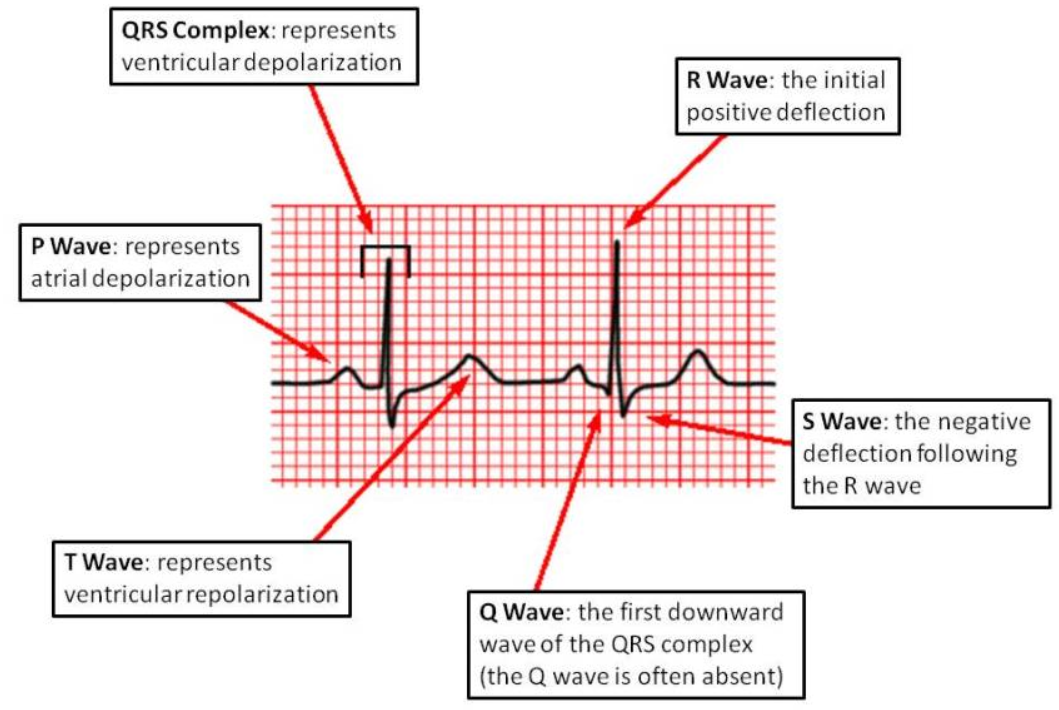
\includegraphics[width=\textwidth]{wave_and_complex}
		\caption{}
	\end{subfigure}
	\caption{(a)12 Lead ECG. (b) Gelombang dan kompleks pada sinyal ECG.}
	\captionsetup{font={footnotesize}}
	\caption*{sumber: https://meds.queensu.ca/central/assets/modules/ts-ecg/the\_12\_lead\_ecg.html (diakses tanggal 9 Juni 2018)}
	\label{fig:ecg_wave}
\end{figure}

ECG merupakan proses perekaman aktifitas kelistrikan pada jantung menggunakan elektroda yang ditempatkan pada kulit selama periode waktu tertentu.~Elektroda ini berfungsi untuk mendeteksi perubahan elektrik kecil pada kulit yang timbul dari pola elektrofisiologis jantung dari depolarisasi dan repolarisasi setiap detak jantung.~Hal ini sangat umum dilakukan untuk mendeteksi masalah jantung.
Pada 12-lead ECG konvensional, sepuluh elektroda ditempatkan pada anggota tubuh pasien pada permukaan dada.~Besar keseluruhan dari potensi kelistrikan jantung kemudian diukur melalui 12 sudut yang berbeda (Leads) dan dicatat dalam bentuk grafik ---seperti pada Gambar~\ref{fig:ecg_wave}--- selama periode waktu tertentu.~Dengan cara ini, besar keseluruhan serta arah depolarisasi kelistrikan jantung dapat didapatkan pada setiap momen sepanjang siklus jantung.


%\begin{figure}[ht]
%\centering
% 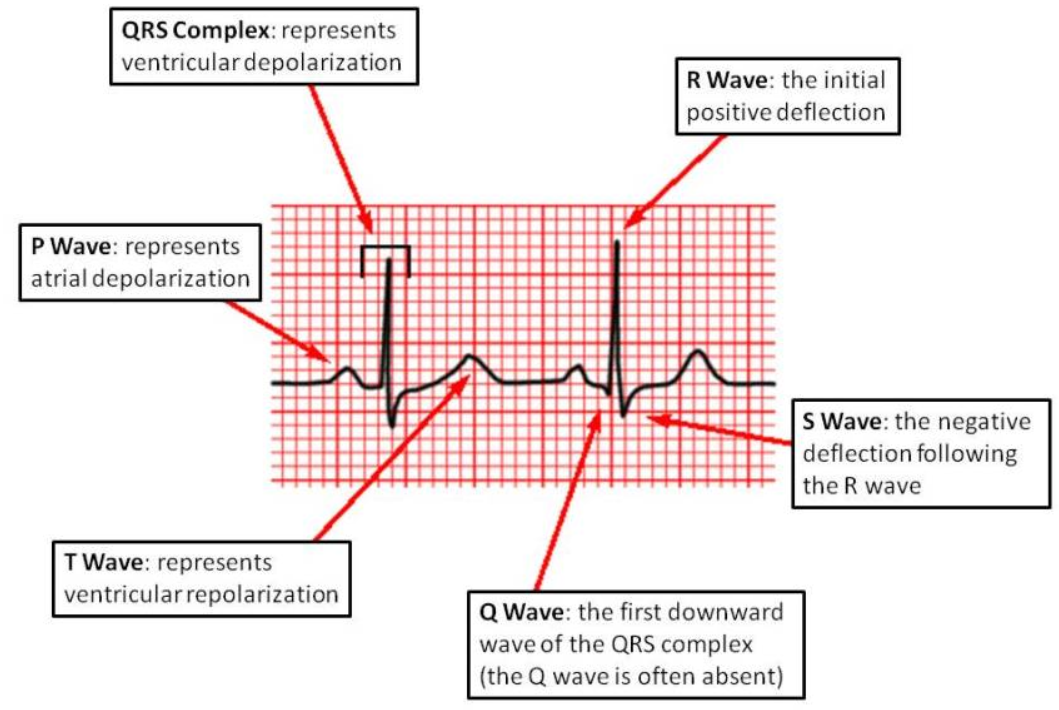
\includegraphics[width=0.6\textwidth]{wave_and_complex}
% \caption{Gelombang dan kompleks pada sinyal ECG.}
%  \captionsetup{font={footnotesize}}  
%  \caption*{sumber: https://meds.queensu.ca/central/assets/modules/ts-ecg/the\_12\_lead\_ecg.html (diakses tanggal 9 Juni 2018)}
% \label{fig:wave_and_complex}   
%\end{figure}

\section{\textit{Photoplethysmography} (PPG)}

Photoplethysmography (PPG) adalah teknik non-invasif untuk mengukur perubahan volume darah mikrovaskular yang terjadi pada wilayah jaringan (\textit{tissue bed}) di bawah lapisan kulit ---yang disebabkan oleh sifat pulsatil dari sistem sirkulasi darah dikarenakan aktifitas jantung berdetak--- dengan menempatkan iluminasi kecil dan probe deteksi pada permukaan kulit [\citet{Allen2007,Kamal1989}].~Karena merupakan teknik optis, PPG membutuhkan sumber cahaya dan fotodetektor untuk berfungsi.~Sumber cahaya berfungsi untuk menerangi jaringan tubuh dan fotodetektor untuk merasakan variasi  kecil dalam intensitas cahaya yang dipantulkan atau ditransmisikan berkaitan dengan perubahan perfusi dalam volume tertentu [Ugnell dan Öberg \citep{ugnell1995}]. 

\begin{figure}[ht]
	\vspace{0.3em}
	\centering
	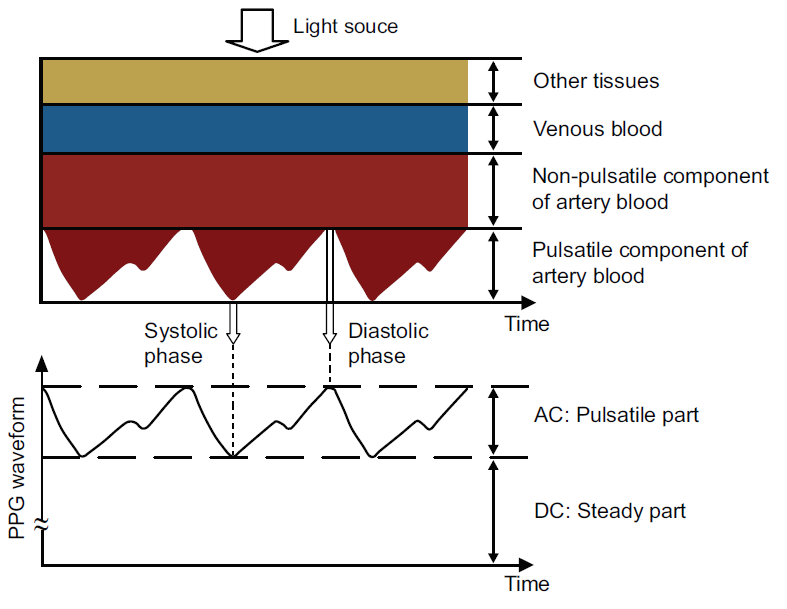
\includegraphics[width=0.7\textwidth]{ppg}
	\caption{Variasi dalam redaman cahaya oleh jaringan tubuh.}
	\captionsetup{font={footnotesize}}  
	\caption*{sumber: Tamura et al. (2014). "Wearable Photoplethysmographic Sensors—Past and Present". \textit{Electronics,} Vol.~3, halaman 283.}
	\label{fig:ppg}   
\end{figure}

Prinsip dasar PPG bergantung pada sensitivitas perubahan panjang gelombang optis pada jaringan darah dan jaringan tubuh lainnya.~Gambar~\ref{fig:ppg} menunjukkan sistem PPG menghasilkan bentuk gelombang yang dapat mewakili perubahan volume darah yang disebabkan oleh detakan jantung dengan mengukur reflektansi atau transmisi sumber cahaya pada kulit.~Metode ini telah terbukti memiliki banyak kegunaan medis dalam pengukuran fitur kardiovaskular seperti denyut jantung, volume darah, saturasi oksigen dan bahkan tingkat respirasi [\citet{Allen2007,charlton2016}].

Komponen pulsatil dari gelombang PPG sering disebut komponen 'AC' dan biasanya memiliki frekuensi fundamentalnya sendiri ---biasanya sekitar 1 Hz--- tergantung pada sinyal denyut jantung seperti pada Gambar~\ref{fig:ecg_and_ppg}.~Komponen AC ditumpangkan ke komponen kuasi-DC besar yang berhubungan dengan jaringan dan volume darah rata-rata.~Komponen DC ini mengalami perubahan secara perlahan karena pengaruh respirasi, aktivitas vasomotorik dan gelombang vasokonstriktor, gelombang \textit{Traube Hering Mayer} (THM) dan juga termoregulasi [\citet{Allen2007}].
\begin{figure}[ht]
	%\vspace{0.5em}
	\centering
	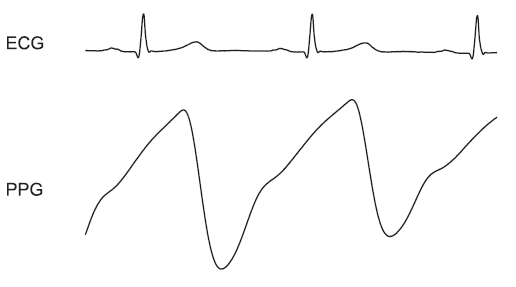
\includegraphics[width=0.4\textwidth]{ecg_and_ppg}
	\caption{Komponen pulsatil (AC) dari sinyal PPG dan sesuai dengan ECG.}
	\captionsetup{font={footnotesize}}  
	\caption*{sumber: Allen, J. (2007). "Photoplethysmography and its application in clinical physiological measurement". \textit{Physiological Measurement,} Vol.~28, No. 3, halaman R3.}
	\label{fig:ecg_and_ppg}   
\end{figure}
\subsection{Wearable \textit{Photoplethysmography} (PPG)}
Metode Wearable PPG telah banyak dikembangkan dan diaplikasikan secara luas serta diperjualbelikan.~Contohnya, pada awal tahun 1990an, \textit{pulse oximetry} digunakan menjadi standar internasional yang dimandatkan untuk monitoring detak jantung selama anestesi [\citet{tremper1989}]. 

\begin{figure}[ht]
	%\vspace{0.5em}
	\centering
	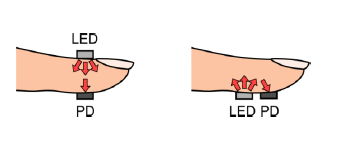
\includegraphics[width=0.3\textwidth]{finger}
	\caption{Penempatan LED dan PD untuk mode transmisi dan reflektansi PPG}
	\captionsetup{font={footnotesize}}  
	\caption*{sumber: Tamura et al. (2014). "Wearable Photoplethysmographic Sensors—Past and Present". \textit{Electronics,} halaman 285.}
	\label{fig:finger}   
\end{figure}

Menurut \citet{Tamura2014}, Wearable PPG memiliki dua mode ---transmisi dan reflektansi--- seperti yang ditunjukkan pada Gambar~\ref{fig:finger}.~Dalam mode transmisi, cahaya yang ditransmisikan melalui medium dideteksi oleh \textit{Photodetector} (PD) yang berlawanan dengan sumber \textit{Light Emitting Diode} (LED), sementara dalam mode reflektansi, PD mendeteksi cahaya yang kembali tersebar atau dipantulkan dari jaringan, tulang dan / atau pembuluh darah.~Mode transmisi mampu memperoleh sinyal yang relatif bagus, tetapi daerah pengukuran mungkin terbatas.~Agar pengukuran efektif, sensor harus ditempatkan pada tubuh di tempat cahaya yang ditransmisikan dapat dengan mudah dideteksi, seperti ujung jari, septum hidung, pipi, lidah, atau daun telinga.~Penempatan sensor pada septum hidung, pipi atau lidah hanya efektif di bawah anestesi.~Pada Tabel \ref{table:wearable_PPG} disajikan penelitian yang menggunakan wearable PPG.

\begin{table}[ht]
	\vspace{0.3em}
	\caption{Daftar Penelitian Dengan Wearable PPG}
	%	\vspace{0.3em}
	\centering
	\label{table:wearable_PPG}
	\resizebox{\textwidth}{!}{%
		\begin{tabular}{| c  c  c  c |}
			\hline 
			Referensi & transmisi/reflektansi & Pengukuran & Letak\\
			\hline
			\citet{Mendelson2006} & reflektansi & HR & Pergelangan tangan \& dahi\\
			\hline
			\citet{Renevey2001} & reflektansi & HR & Pergelangan tangan\\
			\hline
			\citet{Rhee2001} & transmisi & HR & jari manis\\
			\hline
			\citet{Yang1998} & transmisi & HR \& SpO2 & jari manis\\
			\hline
		\end{tabular} 
	}
	\captionsetup{font={footnotesize}}
	\caption*{sumber: Sun, Y. and Thakor, N. (2016). "Photoplethysmography revisited: from contact to noncontact, from point to imaging". \textit{IEEE Transactions on Biomedical Engineering,} Vol.~63, No. 3, halaman 466.}
\end{table}
Menurut Sun dan Thakor \citep{sun2016}, meskipun aplikasi dari PPG luas, terdapat beberapa hal signifikan yang membatasi kegunaan dan pengembangan metode PPG konvensional diantaranya :

\begin{itemize}
	\item \textbf{Pengukuran titik}.~Sensor PPG hanya dapat memantau perubahan dinamis volume darah pada satu tempat / titik per probe.
	\item \textbf{Kontak saat pengukuran}.~Untuk pengukuran yang akurat, sensor PPG konvensional harus melekat kuat pada kulit, yang membatasi kepraktisan dalam situasi seperti diagnosa luka (luka bakar / ulkus / trauma) dan evaluasi penyembuhan kulit atau ketika gerakan bebas diperlukan.
	\item \textbf{Gangguan \textit{motion artifact}}.~PPG rentan terhadap kerusakan sinyal yang diinduksi oleh gerakan.~Hal itu telah dibuktikan secara klinis bahwa artefak gerak (\textit{motion artifact}) dapat menyebabkan kesalahan dalam respons pulsa oximeter.
\end{itemize}

%\subsection{PPG Berbasis Kamera}

\subsection{Non-Wearable \textit{Photoplethysmography} (PPG)}

Pengenalan kamera digital untuk sistem pemantauan dan diagnosis pencitraan klinis, keinginan untuk mengurangi pembatasan fisik, dan kemungkinan wawasan baru yang mungkin berasal dari pencitraan perfusi dan pemetaan mendasari pengembangan teknologi PPG konvensional menjadi \textit{vision-based PPG} (PPG berbasis kamera).~\textit{Image Photoplethysmography} (iPPG) atau PPG berbasis kamera adalah metode non-kontak yang dapat mendeteksi gelombang denyut jantung yang dihasilkan melalui pengukuran perfusi darah perifer [Sun dan Thakor \citep{sun2016}].~
\newpage
\begin{figure}[ht]
	%\vspace{0.5em}
	\centering
	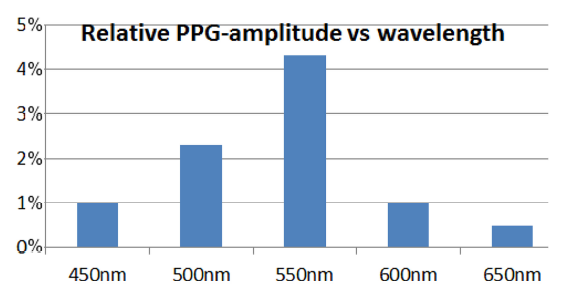
\includegraphics[width=0.6\textwidth]{wavelength}
	\caption{Amplitudo relatif PPG terhadap panjang gelombang PPG berdasarkan penelitian \citet{Crowe1992}}
	\captionsetup{font={footnotesize}}  
	\caption*{sumber: de Haan, G. and Jeanne, V. (2013). "Robust pulse rate from chrominance-based rppg". \textit{IEEE Transactions on Biomedical Engineering,} Vol.~60, No. 10, halaman 2878.}
	\label{fig:wavelength}   
\end{figure}

Pada dasarnya teknik PPG berbasis kamera ini memiliki keuntungan dari fakta bahwa variasi dari penyerapan optis pada kulit manusia bergantung pada panjang gelombang yang digunakan, seperti yang ditunjukkan pada Gambar~\ref{fig:wavelength}.~Perubahan gerakan kulit relatif terhadap sensor, di sisi lain, sebagian besar mempengaruhi intensitas cahaya yang dipantulkan atau ditransmisikan oleh kulit tanpa memperhatikan panjang gelombang [de Haan dan Jeanne \citep{deHaan2013}].~\citet{Verkruysse2008} menemukan bahwa sinyal PPG memiliki kekuatan relatif yang berbeda dalam 3 kanal warna (RGB) dari video pada kamera yang ditujukan ke kulit manusia.~Beberapa penelitian sebelumnya menggunakan \textit{non-wearable sensor} PPG disajikan pada Tabel \ref{table:vision_PPG}.

%Beberapa penelitian sebelumnya menggunakan \textit{non-wearable sensor} PPG contohnya kamera [de Haan dan Jeanne \citep{deHaan2013}, \citet{Estepp2014,lazaro2014,Mirmo2016,nam2014,Poh2010,Poh2011,Wu2000}] menggunakan metode yang beragam untuk mengolah sinyal PPG yang didapat.

\begin{table}[ht]
	\vspace{0.5em}
	\caption{Daftar Penelitian \textit{Non-Wearable Vision Based} PPG}
	%	\vspace{0.3em}
	\centering
	\label{table:vision_PPG}
	\resizebox{\textwidth}{!}{%
		\begin{tabular}{|l c  c  c  c l|}
			\hline 
			Referensi & Kamera && Pengukuran && Sumber cahaya\\
			\hline
			de Haan dan Jeanne \citep{deHaan2013} & CCD && HR && Lampu studio\\
			\hline
			\citet{Estepp2014}* & CCD && HR && Bola lampu\\
			\hline
			\citet{kong2013} & CCD && HR, BR, \& SpO2 && Cahaya sekitar\\
			\hline
			\citet{Poh2010,Poh2011} & Webcam && HR, BR, \& HRV && Cahaya sekitar\\
			\hline
			\citet{RubinsteinPhDThesis2014} & DC && HR && Cahaya sekitar\\
			\hline
			\citet{Scully2012} & Ponsel && HR, BR, \& SpO2 && LED putih\\
			\hline
			\citet{Verkruysse2008} & DC && HR, BR, \& Perfusi && Cahaya sekitar\\
			\hline
		\end{tabular} 
	}
	\vspace{0ex}
	\raggedright{ 
	Catatan: CCD = \textit{Charge Coupled Device}; DC = \textit{Digital Camera}; * = Berjalan dalam mode kontak tanpa penekanan tambahan.}
	\captionsetup{font={footnotesize}}
	\caption*{sumber: Sun, Y. and Thakor, N. (2016). "Photoplethysmography revisited: from contact to noncontact, from point to imaging". \textit{IEEE Transactions on Biomedical Engineering,} Vol.~63, No. 3, halaman 468.}
\end{table}
%\section{Metode Pengolahan \textit{non-Wearable Sensor} PPG}
\section{\textit{Independent Component Analysis} (ICA)}

\begin{figure}[ht]
	\vspace{0.5em}
	\centering
	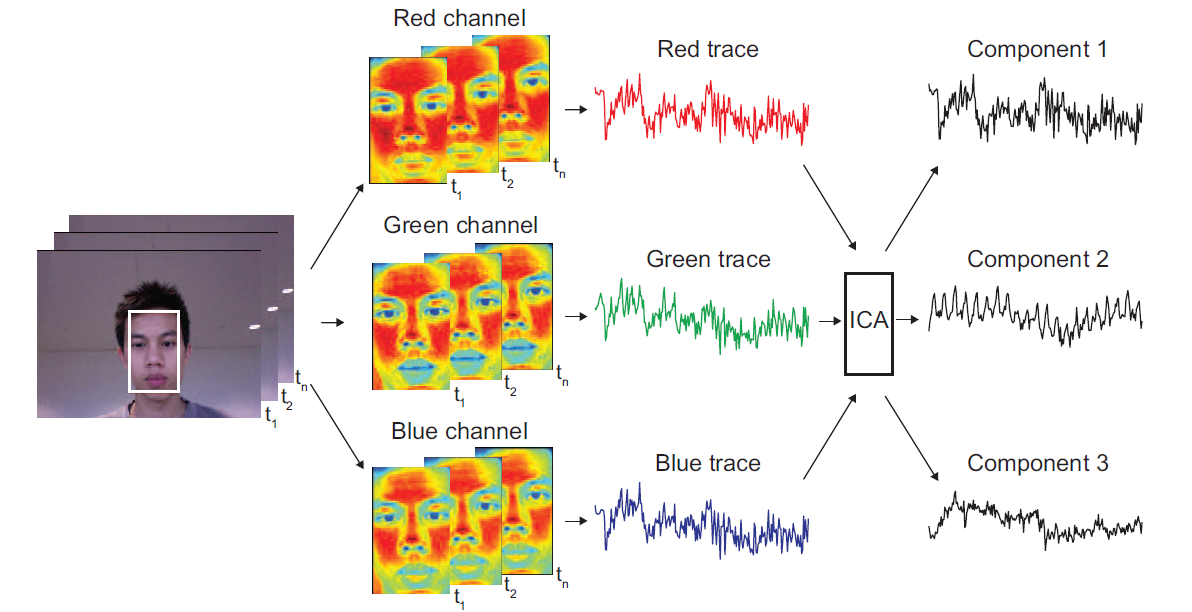
\includegraphics[width=\textwidth]{ICA}
	\caption{Aplikasi Metode ICA untuk memperoleh gelombang PPG}
	\captionsetup{font={footnotesize}}  
	\caption*{sumber: Poh et al, 2010. "Non-contact, automated cardiac pulse measurements using video imaging and blind source separation". \textit{Opt. Express,} Vol.~18, No. 10, halaman 10767.}
	\label{fig:ICA}   
\end{figure}

Salah satu teknik untuk menghilangkan gangguan (\textit{noise}) dari sinyal fisiologis adalah dengan menggunakan \textit{Blind Source Separation} (BSS).~BSS mengacu pada pemulihan sinyal yang tidak teramati atau sumber dari gabungan sinyal yang tidak diketahui sebelumnya bagaimana proses terbentuknya.~Biasanya, hasil pengamatan diperoleh dari output satu set sensor, di mana setiap sensor menerima kombinasi sinyal sumber yang berbeda.~Ada beberapa metode BSS, salah satunya adalah \textit{Independent Component Analysis} (ICA).~ICA adalah teknik untuk mengungkap sinyal sumber independen dari serangkaian pengamatan yang terdiri dari campuran linier dari sumber yang mendasarinya.~Dalam penelitian \citet{Poh2010,Poh2011}, sinyal sumber dasar adalah gelombang denyut jantung yang menyebar ke seluruh tubuh.~Perubahan volumetrik pembuluh darah di area wajah selama siklus kerja jantung memodifikasi panjang dari garis edar cahaya sekitar yang kemudian mengakibatkan perubahan jumlah cahaya yang dipantulkan yang menunjukkan waktu aktifitas kardiovaskular.~Dengan merekam video di daerah wajah menggunakan webcam, sensor warna RGB menangkap campuran sinyal PPG yang dipantulkan bersama dengan sumber lain dari fluktuasi cahaya karena artefak seperti gerak dan perubahan dalam kondisi pencahayaan sekitar.~Mengingat bahwa tingkat penyerapan hemoglobin berbeda pada rentang spektral yang terlihat dan dekat-inframerah [\citet{Zijlstra1991}], setiap sensor warna merekam campuran sinyal sumber asli dengan bobot yang sedikit berbeda.

ICA dapat diterapkan untuk memisahkan data PPG dari artefak gerak, cahaya sekitar (\textit{ambient light}) dan gangguan lain dalam kondisi lingkungan gerak rendah.~Penggunaan ICA menarik karena tidak memerlukan pengetahuan seebelumnya dari sistem.~Namun, ICA mengasumsikan bahwa semua pasangan komponen sinyal sumber saling independen.~Penting untuk menilai kemandirian statistik dari komponen sumber dalam data PPG, terutama jika ICA harus diterapkan dalam lingkungan pemantauan rawat jalan, di mana artefak gerakan dapat memiliki efek substansial pada kualitas data yang diterima dari sensor berbasis cahaya [\citet{Tamura2014}].

\section{\textit{Principle Component Analysis} (PCA)}
Pemfilteran adaptif yang dikombinasikan dengan peningkatan desain mekanik dan konfigurasi probe meningkatkan akurasi sinyal PPG yang dihasilkan [\citet{Rhee2001}].~Kekokohan gerakan (\textit{motion robustness}) dapat diperoleh dengan menggunakan sinyal referensi gerakan yang akurat dari (\textit{low-noise}) akselerometer tiga dimensi (3D), bersama dengan penginderaan inframerah (IR) saluran ganda.~Pemodelan nonlinier dan keragaman spasial dari sensor dapat digunakan untuk menghapus kontribusi gerakan ---artefak gerak--- dalam sinyal optik dan kontribusi timbal balik pada masing-masing saluran.~\textit{Principle Component Analysis} (PCA) ---yang juga merupakan bagian dari metode BSS--- memanfaatkan korelasi spasial dan temporal di antara dan di dalam gangguan (noise) sinyal yang diamati.~Konsep dasar dari pengurangan gangguan berbasis PCA adalah untuk mengamati gangguan data dalam ruang dimensi-m (\textit{m-dimensional space}) yang besar dari koordinat yang tertunda.~Karena gangguan diasumsikan sebagai sesuatu yang tidak tentu membuatnya dapat berada di setiap aspek secara merata dalam cakupan ruang tertentu.~Sebaliknya, dinamika penetapan sistem pokok untuk membatasi lintasan sinyal yang berguna menjadi sub-ruang dimensi yang lebih rendah (p < m).~Oleh karena itu, ruang Eigen (\textit{Eigenspace}) dari beragam gangguan yang diamati dipisahkan menjadi gangguan (\textit{noise}) dan subruang sinyal dan gangguan.

%\subsection{Periodic Moving Average Filter (PMAF)}
%Metode rata-rata bergerak (\textit{Moving Average Filter}) umumnya digunakan untuk mengurangi artefak gerak dan bekerja dengan baik dalam jangkauan artefak yang terbatas. Namun, metode ini tidak dapat memperhitungkan perubahan gerak mendadak. Filter PMAF berdasarkan sinyal PPG yang bersifat kuasi-periodik, membagi sinyal PPG ke dalam beberapa periode dan melakukan sampel ulang pada setiap periode. Dengan begitu metode PMAF dapat menghilangkan artefak gerak tanpa menurunkan kualitas sinyal (Lee et al, 2007). Gangguan in-band (\textit{in-band noise}) terjadi ketika spektrum artefak gerak dan sinyal PPG tumpang tindih secara signifikan. Namun, tidak disarankan untuk menggunakan teknik penyaringan frekuensi tetap (\textit{fixed-frequency}) untuk menghilangkan artefak gerak karena gangguan in-band dan spektrum frekuensi yang tumpang tindih dalam sinyal PPG. Sebaliknya, artefak gerak dapat dihilangkan menggunakan bank filter dan filter yang sesuai yang terdiri dari beberapa pita frekuensi (Lee et al, 2004). Dalam hal ini, filter adaptif menunjukkan banyak perbedaan dan kesalahan dikarenakan variasi amplitudo selama konvergensi ketika mengukur PPG secara real-time, sedangkan MAF menunjukkan output yang lebih stabil (Lee et al, 2004).

%\subsection{Fourier Analysis}
%Penggunaan deret Fourier hanya berlaku untuk sinyal yang periodik, oleh karena itu tidak dapat diterapkan secara langsung pada sinyal PPG karena sifatnya yang tidak statis dan kuasi-periodik. Untuk mengatasi masalah tersebut analisa deret Fourier dapat diterapkan dengan basis siklus demi siklus. Dalam hal ini, data yang diperoleh pertama-tama disaring dengan menggunakan filter Savitzky-Golay (SG) untuk menghilangkan gangguan frekuensi tinggi. Setelah gangguan dihilangkan, analisa deret fourier siklus demi siklus (\textit{cycle-by-cycle Fourier series}) dilakukan dan sinyal PPG (IR dan merah) direkonstruksi secara siklus demi siklus. Hasil penelitian (Reddy et al, 2009) telah membuktikan keberhasilan metode yang digunakan. Selain itu, hasil penelitian juga menunjukkan bahwa artefak gerak yang diinduksi oleh gerakan pasien dapat dilemahkan setidaknya 35 dB yang mengakibatkan pengurangan kesalahan pengukuran sinyal PPG dari 37\% menjadi 3\% menggunakan teknik yang diusulkan.

%\subsection{Kalman Filter}
%Pada penelitian (Lee et al, 2010) penggunaan Kalman filter dapat digunakan untuk memperkirakan pengurangan artefak gerak dan telah terbukti memberikan informasi yang akurat dari sinyal PPG yang direkonstruksi. Dengan menggunakan struktur data khusus dalam Kalman filter estimasi sinyal PPG yang sebenarnya dapat diperoleh. Pada studi (Seyeditabaii, S. dan Seyedtabaii, L., 2008) gerakan jari disimulasikan dan digunakan sebagai referensi gangguan. Sinyal PPG yang terkontaminasi oleh gangguan digunakan sebagai sinyal utama dan algoritma yang diusulkan mampu mengekstrak sinyal utama dari gangguan dalam pita frekuensi yang sama, tidak seperti metode filter yang konvensional.

\section{\textit{Eulerian Video Magnification} (EVM)}

\textit{Eulerian Video Magnification} (EVM) merupakan metode komputasional untuk menghitung dan juga menjadi metode untuk menguatkan proses perubahan kecil/halus ke sinyal data video.~Metode ini digunakan untuk menampilkan perubahan warna ataupun pergerakan translasional yang sulit atau tidak dapat dilihat dengan kasat mata.~EVM menggunakan rangkaian video standar sebagai masukan (\textit{input}) kemudian menerapkan dekomposisi spasial diikuti dengan pemfilteran sementara (\textit{temporal filtering}) terhadap frame.~Sinyal yang dihasilkan kemudian akan dimagnifikasi untuk mengungkap informasi yang tersembunyi.~Pada penelitian \citet{Wu2012}, metode EVM dapat memvisualisasikan aliran darah saat melewati wajah dan juga mengungkap pergerakan kecil/halus.~Pendekatan dasar yang digunakan adalah untuk memperhatikan rangkaian waktu (\textit{time series}) dari nilai suatu warna pada setiap lokasi ---spasial berupa piksel--- dan memperkuat variasi dalam suatu pita frekuensi waktu yang diberikan.
\begin{figure}[ht]
	\centering
	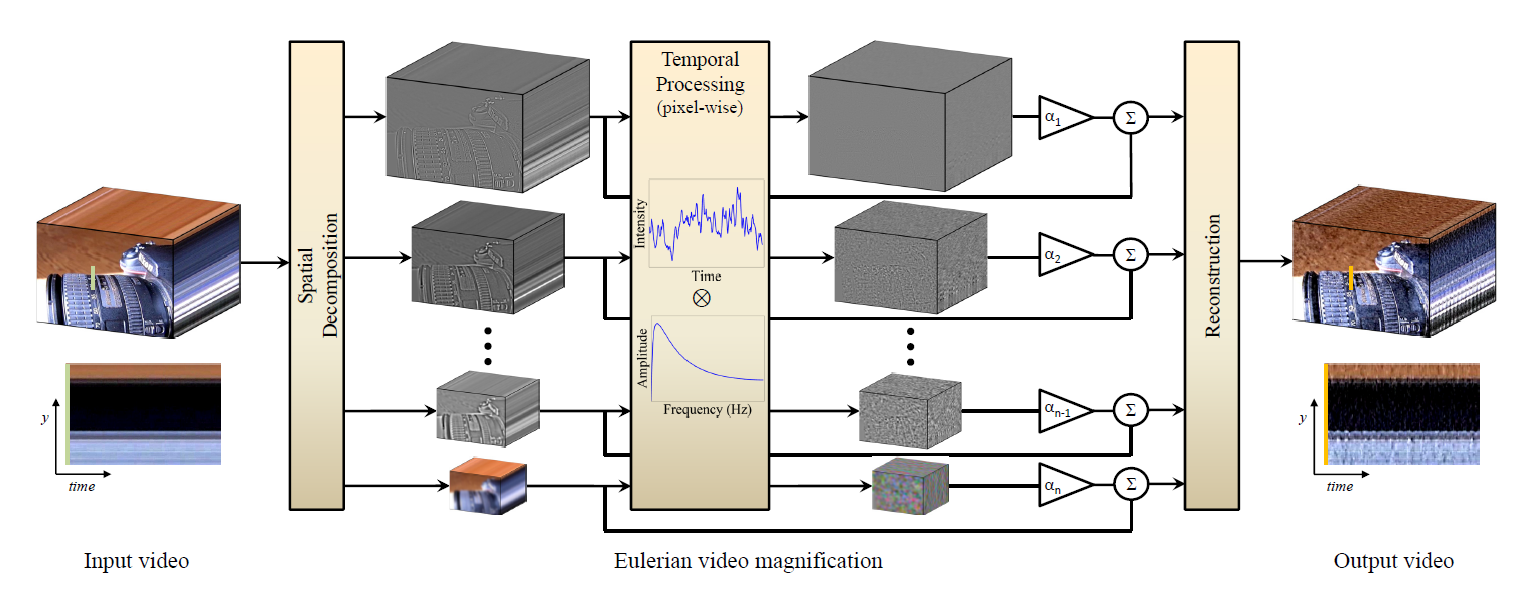
\includegraphics[width=\textwidth]{EVM}
	\caption{Kerangka Kerja Metode EVM}
	\captionsetup{font={footnotesize}}  
	\caption*{sumber: Wu et al. (2012). "Eulerian Video Magnification for Revealing Subtle Changes in the World". \textit{ACM Trans. Graph. (Proceedings SIGGRAPH 2012),} Vol.~31, No. 4, halaman 65:1.}
	\label{fig:EVM}   
\end{figure}

Melalui proses deteksi dan perbesaran variasi warna halus/kecil ---0,5 unit intensitas dalam skala 8 bit--- dari kulit manusia yang disebabkan oleh aliran darah, HR dapat diekstraksi secara baik dari video RGB standar di mana setiap piksel mencatat nilai intensitas antara 0-255.~Biasanya, kualitas sinyal pulsa yang diekstraksi dari titik yang berbeda pada wajah maupun bagian tubuh yang lain dapat bervariasi.~Hal ini dikarenakan amplitudo sinyal dapat dimodulasi sesuai dengan kepadatan pembuluh darah perifer, serta karena adanya kontras spasial yang tinggi dari tubuh atau wajah yang membuat lebih sulit untuk mengekstrak sinyal.~Selain itu juga terdapat kemungkinan adanya kesalahan dalam mendeteksi puncak pada sinyal bandpass yang digunakan.
Perbedaan penting dari metode pengukuran PPG menggunakan kamera sebelumnya [\citet{kong2013,lazaro2014,lewandowska2011,Mirmo2016,Poh2010,Poh2011,Sun2012,Verkruysse2008}] menggunakan nilai rata-rata piksel di seluruh wilayah wajah, sementara metode EVM hanya dengan mengamati daerah pulsatil di wajah yang akan digunakan untuk mengestimasi nilai HR. 

\subsection{\textit{Space-time Video Processing}}
Meninjau wilayah lokal yang tetap dalam sebuah video.~Perubahan warna di wilayah lokal dapat dikaitkan dengan salah satu dari dua sebab yang memungkinkan: (a) objek statis di dalam kawasan telah berubah warna, dan (b) objek di wilayah tersebut telah berpindah, dalam kejadian di mana wilayah tersebut sekarang mungkin memuat bagian yang berbeda dari objek yang ada sebelumnya, atau objek yang berbeda sama sekali.~Mengamplifikasi perubahan warna tersebut secara lokal dan mengembalikannya ke dalam video akan membuatnya lebih terlihat oleh mata manusia.

\citet{RubinsteinPhDThesis2014} menggabungkan pemrosesan spasial dan temporal untuk mempertegas perubahan temporal yang halus dalam suatu video.~Proses tersebut diilustrasikan pada Gambar~\ref{fig:EVM}.~Hal pertama yang dilakukan adalah menguraikan urutan video ke dalam pita frekuensi spasial yang berbeda.~Pita-pita frekuensi tersebut mungkin dimagnifikasi secara berbeda karena (a) mereka mungkin menunjukkan rasio signal-to-noise yang berbeda, atau (b) mereka mungkin mengandung frekuensi spasial yang penaksiran linearnya tidak berlaku digunakan dalam \textit{Eulerian Motion Magnification} (sub-BAB \ref{ssec:EMM}).~Besaran amplifikasi dikurangi untuk pita-pita frekuensi tertentu untuk mengurangi atau menekan artefak gerak.~Proses tersebut umumnya dilakukan dengan menggunakan perhitungan piramida Laplacian penuh oleh Burt dan Adelson \citep{burt1983}.

Pemrosesan temporal pada setiap pita spasial dilakukan dengan mempertimbangkan rangkaian waktu yang sesuai dengan nilai piksel dalam pita frekuensi dan menerapkan bandpass filter untuk mengekstrak pita frekuensi yang dibutuhkan.~Sebagai contoh, rentan frekuensi dapat dipilih dalam 0.4-4 Hz yang mengimplementasikan 24-240 denyut per menit.~Gambar~\ref{fig:compare} menunjukkan rentan nilai frekuensi dan piksel-piksel yang diwakili.~Rentan frekuensi tersebut dapat diatur dan dapat dipersempit di sekitar nilai data denyut nadi ketika telah berhasil diekstrak.~Pemrosesan temporal seragam untuk semua tingkat spasial, dan untuk semua piksel dalam setiap level.


\subsection{\textit{Eulerian Motion Magnification}} \label{ssec:EMM}
Menurut \citet{RubinsteinPhDThesis2014}, terdapat banyak piksel di daerah wajah terutama yang berada dalam wilayah kontak spasial tinggi tidak memberikan informasi aktifitas jantung yang dapat diandalkan, seperti yang terlihat pada Gambar~\ref{fig:compare}.~Dengan begitu, rata-rata yang didapatkan atas daerah deteksi seperti yang dilakukan dalam penelitian sebelumnya [\citet{Poh2010,Poh2011}] dapat mengurangi rasio \textit{signal-to-noise} (SNR) dan keakuratan perkiraan HR.


\begin{figure}[ht]
	\vspace{0.5em}
	\centering
	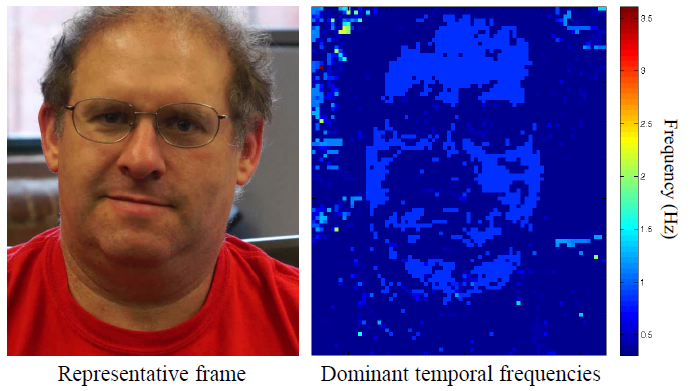
\includegraphics[width=0.8\textwidth]{Compare}
	\caption{Visualisasi frekuensi temporal yang dominan}
	\captionsetup{font={footnotesize}}  
	\caption*{sumber: M. Rubinstein. (2014). "Analysis and visualization of temporal variations in video". PhD thesis, halaman 97.}
	\label{fig:compare}   
\end{figure}

Untuk menjelaskan hubungan antara pemrosesan sementara dan pembesaran gerakan, \citet{Wu2012} mempertimbangkan kasus sederhana dari sinyal 1D yang menjalani gerakan translasi.~Analisis ini merupakan generalisasi langsung ke gerak translasi lokal dalam 2D.
Menggunakan \(I(x; t)\) untuk menunjukkan intensitas gambar pada posisi \(x\) dan waktu \(t\).~Karena gambar mengalami gerakan translasi, intensitas pengamatan dapat diekspresikan dengan fungsi perpindahan \(\delta (t)\), sehingga \({I(x; t)  =  f(x  +  (t))}\) dan \({I(x; 0)  =  f(x)}\).~Tujuan dari pembesaran gerakan adalah untuk mensintesis sinyal
%\begin{spacing}{0.9}
\begin{equation}\label{eq:2.1}
\begin{aligned}
\hat {I}(x;t) = f(x + (1 + \alpha )\delta (t))
\end{aligned}
\end{equation}
Untuk faktor amplifikasi disimbolkan sebagai \(\alpha \).\newline
%\end{spacing}

Dengan asumsi bahwa gambar dapat didekati dengan menggunakan orde pertama deret Taylor sehingga gambar ditulis dalam waktu \(t\), \(f(x + (1 + \alpha )\delta (t))\) dalam ekspansi orde pertama Taylor terhadap \(x\), sebagai
%\begin{spacing}{0.9}
\begin{equation} \label{eq:2.2}
\begin{aligned}
I(x; t) \approx f(x) + \delta {\rm{(}}t{\rm{)}}\frac{{\partial f(x)}}{{\partial x}}.
\end{aligned}
\end{equation}
%\\
%\end{spacing}

Misalkan \(B(x; t)\) merupakan hasil penerapan filter bandpass ---dengan jangkauan frekuensi yang luas--- sementara pada \(I(x; t)\) di setiap posisi \(x\) (kecuali pada \(f(x)\) dalam Persamaan (\ref{eq:2.2})).~Untuk saat ini, asumsikan sinyal gerak \(\delta (t)\) berada di dalam passband dari filter bandpass sementara (\textit{temporal bandpass filter}) ---asumsi akan dilonggarkan nanti---, sehingga
%\begin{spacing}{0.9}
\begin{equation} \label{eq:2.3}
\begin{aligned}
B(x; t)  = \delta {(t)}\frac{{\partial f(x)}}{{\partial x}}.
\end{aligned}
\end{equation}
%\\
%\end{spacing}


Dalam prosesnya, sinyal handpass kemudian diamplifikasi dengan \(\alpha \) dan menambahkannya kembali ke \(I(x; t)\), menghasilkan sinyal yang telah diproses
%\begin{spacing}{0.9}
\begin{equation} \label{eq:2.4}
\begin{aligned}
{\tilde I(x; t)  =  I(x; t)  +  }\alpha {B(x; t)}.
\end{aligned}
\end{equation}
%\\
%\end{spacing}


Dengan menggabungkan Persamaan (\ref{eq:2.2}), (\ref{eq:2.3}), dan (\ref{eq:2.4}), sehingga didapatkan 
%\begin{spacing}{0.9}
\begin{equation} \label{eq:2.5}
\begin{aligned}
\tilde I(x; t) \approx {f(x)  +  (1 + }\alpha)\delta {(t)}\frac{{\partial f(x)}}{{\partial x}}.
\end{aligned}
\end{equation}
%\\
%\end{spacing}

Dengan mengasumsikan ekspansi orde pertama Taylor berlaku untuk mengamplifikasi gangguan yang lebih besar \((1 +\alpha)\delta{(t)}\), amplifikasi dari sinyal bandpassed sementara dengan magnifikasi gerakan dapat direlasikan.~Luaran yang diproses adalah
%\begin{spacing}{0.9}
\begin{equation} \label{eq:2.6}
\begin{aligned}
\tilde I(x; t) \approx f(x  +  (1  + \alpha )\delta (t)).
\end{aligned}
\end{equation}
Ini menunjukkan bahwa pengolahan perbesaran gerakan ---perpindahan spasial  \(\delta (t)\) dari citra lokal \(f(x)\) pada waktu \(t\)--- telah dimagnifikasi dengan magnitudo \((1+\alpha)\).\\
%\end{spacing}

Proses ini diilustrasikan untuk satu gelombang sinusoid pada Gambar~\ref{fig:Sinus}.~Pada gelombang kosinus frekuensi rendah dan perpindahan yang relatif kecil \(\delta (t)\), ekspansi deret Taylor orde pertama berfungsi sebagai pendekatan yang baik untuk sinyal yang ditranslasi pada waktu \(t+1\).~Ketika menguatkan sinyal sementara dengan \(\alpha\) dan menambahkannya kembali ke \(I(x; t)\), diperkirakan gelombang tersebut ditranslasi dengan \((1  + \alpha )\delta\).

\begin{figure}[ht]
	\vspace{0.5em}
	\centering
	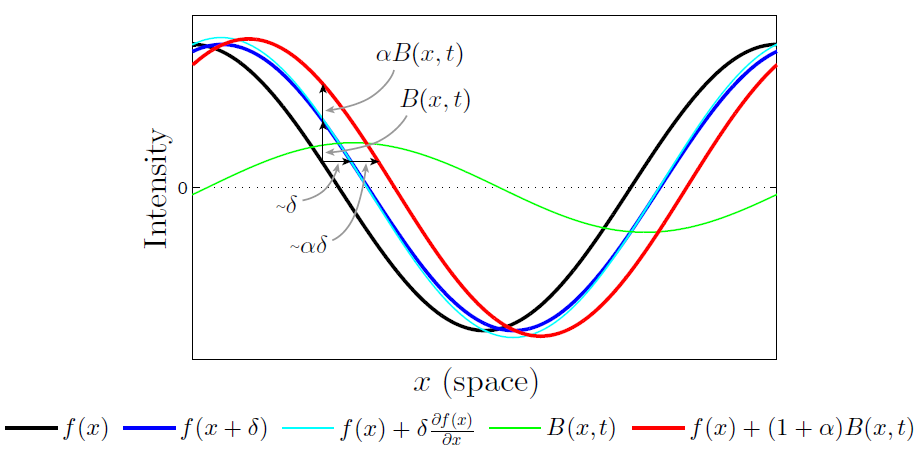
\includegraphics[width=\textwidth]{Sinus}
	\caption[Pemfilteran temporal untuk memperkirakan translasi spasial]{Pemfilteran temporal untuk memperkirakan translasi spasial.~Hasil pemfilteran ditunjukkan dalam sinyal 1D, akan tetapi hal tersebut berlaku juga untuk sinyal 2D.~Sinyal input ditampilkan pada dua waktu instan: \(I(x; t) = f(x)\) pada waktu \(t\) dan \(I(x; t+1) = f(x + \delta)\) \(t+1\).~Urutan pertama ekspansi deret Taylor dari \(I(x; t+1)\) terhadap \(x\) mendekati sinyal yang ditranslasi dengan baik.~Bandpass sementara diamplifikasi dan ditambahkan ke sinyal asli untuk menghasilkan translasi yang lebih besar.~Dalam contoh ini \(\alpha=1\) memperbesar gerakan sebesar 100\%, dan filter temporal merupakan filter beda hingga (\textit{finite difference}) mengurangkan dua kurva.}
	\captionsetup{font={footnotesize}}  
	\caption*{sumber: Wu et al. (2012). "Eulerian Video Magnification for Revealing Subtle Changes in the World". \textit{ACM Trans. Graph. (Proceedings SIGGRAPH 2012),} Vol.~31, No. 4, halaman 65:3.}
	\label{fig:Sinus}   
\end{figure}

Untuk lebih lengkap, kembali dalam kasus yang lebih umum di mana \(\delta (t)\) tidak sepenuhnya berada di dalam passband dari filter temporal.~Dalam hal ini \({\delta _k}(t)\) diindeks oleh k, mewakili komponen spektral temporal yang berbeda \(\delta (t)\).~Setiap \({\delta _k}(t)\) akan dilemahkan oleh filter temporal berdasarkan faktor \({\gamma _k}\).~Hal ini menghasilkan sinyal bandpass,
%\begin{spacing}{0.9}
\begin{equation} \label{eq:2.7}
\begin{aligned}
B(x; t) = \sum\limits_k^{} {{\gamma _k}{\delta _k}(t)\frac{{\partial f(x)}}{{\partial x}}}
\end{aligned}
\end{equation}
%\\
%\end{spacing}
%
(bandingkan dengan Persamaan (\ref{eq:2.3})).~Lantaran perkalian dalam Persamaan (\ref{eq:2.4}), frekuensi temporal yang bergantung redaman dapat diartikan sebagai faktor pembesaran gerak yang bergantung pada frekuensi \({\alpha _k} = {\gamma _k}\alpha\), menghasilkan luaran magnifikasi gerak,
%\begin{spacing}{0.9}
\begin{equation} \label{eq:2.8}
\begin{aligned}
\tilde I(x;t) \approx f(x + \sum\limits_k {(1 + {\alpha _k})} {\delta _k}(t))
\end{aligned}
\end{equation}
%\\
%\end{spacing}

Hasilnya adalah seperti yang diharapkan untuk analisis linear: modulasi komponen spektral dari sinyal gerak menjadi faktor modulasi dalam faktor amplifikasi gerak \(\alpha _k\), untuk setiap sub-band sementara \(\gamma _k\), dari sinyal gerakan.

